% Quicksort recursion tree (generated by figs_c2ch02.py).
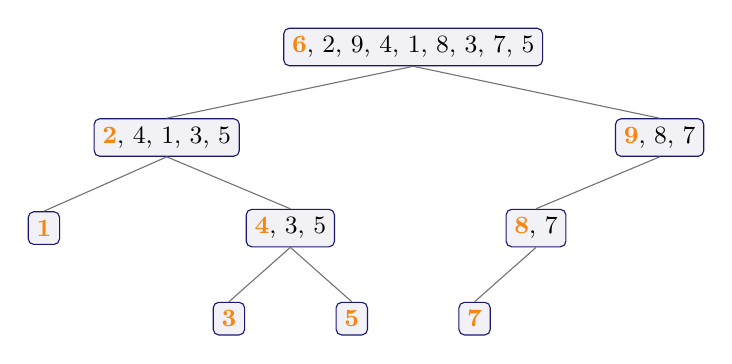
\begin{tikzpicture}[x=1cm,y=1cm,every node/.style={font=\small}]
\node[draw=MidnightBlue,fill=MidnightBlue!6,rounded corners=2pt,inner sep=3pt] (q0) at (6.25,-0.00) {$\textcolor{BurntOrange}{\mathbf{6}},\,2,\,9,\,4,\,1,\,8,\,3,\,7,\,5$};
\node[draw=MidnightBlue,fill=MidnightBlue!6,rounded corners=2pt,inner sep=3pt] (q1) at (3.12,-1.15) {$\textcolor{BurntOrange}{\mathbf{2}},\,4,\,1,\,3,\,5$};
\draw[black!55] (q0.south) -- (q1.north);
\node[draw=MidnightBlue,fill=MidnightBlue!6,rounded corners=2pt,inner sep=3pt] (q2) at (1.56,-2.30) {$\textcolor{BurntOrange}{\mathbf{1}}$};
\draw[black!55] (q1.south) -- (q2.north);
\node[draw=MidnightBlue,fill=MidnightBlue!6,rounded corners=2pt,inner sep=3pt] (q3) at (4.69,-2.30) {$\textcolor{BurntOrange}{\mathbf{4}},\,3,\,5$};
\draw[black!55] (q1.south) -- (q3.north);
\node[draw=MidnightBlue,fill=MidnightBlue!6,rounded corners=2pt,inner sep=3pt] (q4) at (3.91,-3.45) {$\textcolor{BurntOrange}{\mathbf{3}}$};
\draw[black!55] (q3.south) -- (q4.north);
\node[draw=MidnightBlue,fill=MidnightBlue!6,rounded corners=2pt,inner sep=3pt] (q5) at (5.47,-3.45) {$\textcolor{BurntOrange}{\mathbf{5}}$};
\draw[black!55] (q3.south) -- (q5.north);
\node[draw=MidnightBlue,fill=MidnightBlue!6,rounded corners=2pt,inner sep=3pt] (q6) at (9.38,-1.15) {$\textcolor{BurntOrange}{\mathbf{9}},\,8,\,7$};
\draw[black!55] (q0.south) -- (q6.north);
\node[draw=MidnightBlue,fill=MidnightBlue!6,rounded corners=2pt,inner sep=3pt] (q7) at (7.81,-2.30) {$\textcolor{BurntOrange}{\mathbf{8}},\,7$};
\draw[black!55] (q6.south) -- (q7.north);
\node[draw=MidnightBlue,fill=MidnightBlue!6,rounded corners=2pt,inner sep=3pt] (q8) at (7.03,-3.45) {$\textcolor{BurntOrange}{\mathbf{7}}$};
\draw[black!55] (q7.south) -- (q8.north);
\end{tikzpicture}
